\documentclass[ignorenonframetext,]{beamer}
\setbeamertemplate{caption}[numbered]
\setbeamertemplate{caption label separator}{: }
\setbeamercolor{caption name}{fg=normal text.fg}
\beamertemplatenavigationsymbolsempty
\usepackage{lmodern}
\usepackage{amssymb,amsmath}
\usepackage{ifxetex,ifluatex}
\usepackage{fixltx2e} % provides \textsubscript
\ifnum 0\ifxetex 1\fi\ifluatex 1\fi=0 % if pdftex
  \usepackage[T1]{fontenc}
  \usepackage[utf8]{inputenc}
\else % if luatex or xelatex
  \ifxetex
    \usepackage{mathspec}
  \else
    \usepackage{fontspec}
  \fi
  \defaultfontfeatures{Ligatures=TeX,Scale=MatchLowercase}
\fi
\usetheme[]{Frankfurt}
\usecolortheme{crane}
% use upquote if available, for straight quotes in verbatim environments
\IfFileExists{upquote.sty}{\usepackage{upquote}}{}
% use microtype if available
\IfFileExists{microtype.sty}{%
\usepackage{microtype}
\UseMicrotypeSet[protrusion]{basicmath} % disable protrusion for tt fonts
}{}
\newif\ifbibliography
\hypersetup{
            pdftitle={Corporate Relocation and Housing Values},
            pdfborder={0 0 0},
            breaklinks=true}
\urlstyle{same}  % don't use monospace font for urls
\usepackage{graphicx,grffile}
\makeatletter
\def\maxwidth{\ifdim\Gin@nat@width>\linewidth\linewidth\else\Gin@nat@width\fi}
\def\maxheight{\ifdim\Gin@nat@height>\textheight0.8\textheight\else\Gin@nat@height\fi}
\makeatother
% Scale images if necessary, so that they will not overflow the page
% margins by default, and it is still possible to overwrite the defaults
% using explicit options in \includegraphics[width, height, ...]{}
\setkeys{Gin}{width=\maxwidth,height=\maxheight,keepaspectratio}

% Prevent slide breaks in the middle of a paragraph:
\widowpenalties 1 10000
\raggedbottom

\AtBeginPart{
  \let\insertpartnumber\relax
  \let\partname\relax
  \frame{\partpage}
}
\AtBeginSection{
  \ifbibliography
  \else
    \let\insertsectionnumber\relax
    \let\sectionname\relax
    \frame{\sectionpage}
  \fi
}
\AtBeginSubsection{
  \let\insertsubsectionnumber\relax
  \let\subsectionname\relax
  \frame{\subsectionpage}
}

\setlength{\parindent}{0pt}
\setlength{\parskip}{6pt plus 2pt minus 1pt}
\setlength{\emergencystretch}{3em}  % prevent overfull lines
\providecommand{\tightlist}{%
  \setlength{\itemsep}{0pt}\setlength{\parskip}{0pt}}
\setcounter{secnumdepth}{0}

\title{Corporate Relocation and Housing Values}
\author{Benjamin Monticello \textbar{} Fangwen Zhang \textbar{} Humera Durrani}
\date{April 28, 2019}

\begin{document}
\frame{\titlepage}

\begin{frame}{Background}

\begin{figure}
\centering
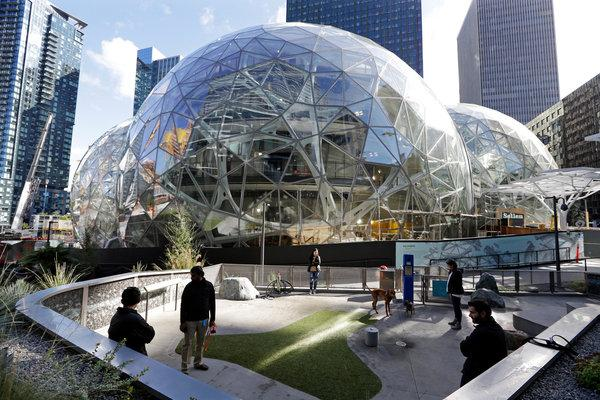
\includegraphics{picture/amazon.jpg}
\caption{Amazon's headquarter in Seattle}
\end{figure}

\end{frame}

\begin{frame}{Background}

\begin{figure}
\centering

\includegraphics{picture/House_price.jpg}
\caption{Unaffordable housing price}
\end{figure}

\end{frame}

\begin{frame}{Problem Statement}

Hypothesis:

Both the announcement of a corporate headquarter relocation and the
opening of the new development will result in a noticeable increase in
local housing prices.

\end{frame}

\begin{frame}{Approach}

Data visualization: Shiny

\begin{itemize}
\tightlist
\item
  Examined median housing value data
\item
  Identify 3-5 companies that are relevant for our work
\end{itemize}

\end{frame}

\begin{frame}{Methods}

\url{Aim:give} users a tool to analyze trends relating to corporate
moves and make that conclusion for themselves.

Methods: - API (Quandl) - Shiny (interactive visualization)

\end{frame}

\begin{frame}{Results}

\href{https://ben-monticello.shinyapps.io/ProjectApp/}{Link to final
app!}

Successfully created a tool that gives users the ability to examine the
relationship between the corporate relocations and housing value trends.

(1)All selected cities have higher median housing values in true value
than the U.S. average - with Chicago, IL nearest to the U.S. average and
Arlington, VA with the greatest difference from the average value.

\end{frame}

\begin{frame}{Results}

(2)Regional housing value stays consistent in its market trajectory
regardless of corporate relocations with cities like Boston and Plano
largely moving in an upward direction and Arlington and Chicago and
Estero for the most part moving in a negative direction.

(3)Many cities across the U.S. are compounded with the opportunities of
an expanding labor market but challenged with a housing market that's
becoming less accessible for those seeking opportunities.

\end{frame}

\begin{frame}{Lessons Learned/Next step}

\end{frame}

\end{document}
